\chapter{Implementierung}
Der jetzige Algorithmus besteht aus vier wichtigen Methoden. Die erste ist die \texttt{try\_fit}-Methode, welche den Einstiegspunkt für den in Kapitel \ref{chapter2} erörterten Algorithmus bildet.
\begin{lstlisting}[language=python,caption={Einstiegspunkt},captionpos=b,label={lst:optimize},escapechar=|,numbers=left]
def optimize(self):
    self.reservations.sort(key=lambda x: x.size, reverse=True)  # sort reservations after size
    self.try_fit()
    self.show_space_used()
\end{lstlisting}
Die von Listing \ref{lst:optimize} gezeigte Methode sortiert erst alle Reservierungen nach ihrer Größe in der Zeitachse. Danach werden die Reservierungen in den Platz einsortiert und von der letzten Methode die Effizienz des Algorithmus ausgegeben.
% Die try_fit-Methode
\begin{lstlisting}[language=python,caption={try\_fit-Methode},captionpos=b,label={lst:tryfit},escapechar=|,numbers=left]
def try_fit(self):
    for i in range(len(self.reservations)):
        interfering_reservations = self.get_reservation_from_tensor(self.reservations[i])
        interfering_reservations.sort(key=lambda element: element.x, reverse=False)  # sort the reservations after x position |\label{tfm:4}|
        x_pos = self.find_first_valid_position(interfering_reservations, self.reservations[i]) |\label{tfm:5}|
        self.reservations[i].x = x_pos

        # only add the reservations which really fit inside the available space
        if x_pos >= 0:
            self.add_reservation_to_tensor(self.reservations[i])
\end{lstlisting}
In der Methode wird jede Reservierung durchgelaufen. Als erstes werden die Reservierungen aus dem Tensor ermittelt, welche mit der neuen Reservierung zusammenstoßen würden. Danach werden die Reservierungen nach ihrer Position sortiert. Dann wird die erste freie Position in dem entstehenden System genommen und der neuen Reservierung zugewiesen. Abschließend wird die Reservierung dem Tensor hinzugefügt, jedoch nur, wenn sie dem Feld hinzugefügt wurde, andernfalls muss sie ignoriert werden. Die interferierenden Reservierungen werden mit der Methode in Zeile 3 ermittelt.
\newpage
% Die Ermittlung der interferierenden Reservierungen
\begin{lstlisting}[language=python,caption={get\_reservation\_from\_tensor-Methode},captionpos=b,label={lst:grft},escapechar=|,numbers=left]
def get_reservation_from_tensor(self, r):
    arr = []

    x_range = self.duration - (r.begin - self.time_range[0])
    x_start = r.begin - self.time_range[0] + 1
    # this must always start at 8 because of this example [8-15] and [9-10] 1 interferes with 2
    y_range = r.ending - self.time_range[0]

    for i in range(x_range):
        for j in range(y_range):
            for reservation in self.tensor[i + x_start][j]:
                arr.append(reservation)

    return arr
\end{lstlisting}
Die Methode gibt einen Array von Reservierungen wieder, welche wegen ihrer Start- und Endzeit mit der neuen Reservierung \texttt{r} interferieren. Als erstes wird ermittelt von wo bis wo auf der X-Achse die Reservierungen gehen, damit sie überschneiden. Dafür werden die beiden Variablen \texttt{x\_range} und \texttt{x\_start} initialisiert und deklariert. \texttt{x\_range} ist dabei die Distanz von dem Startwert bis zur Endzeit des Flohmarkts. Währenddessen ist \texttt{x\_start} der Wert, bei dem der Index startet. Die Variable \texttt{y\_range} hängt von der Endzeit ab und somit inwiefern End- und Startzeit der beiden Reservierungen zusammenhängen. Mit Schleifen können die Felder via Indizes ausgewählt werden. Abbildung \ref{fig:matrix_selected} zeigt wie eine solche Selektion der Reservierungen, welche zeitlich interferieren aussieht.
\begin{figure}[H]
    \centering
    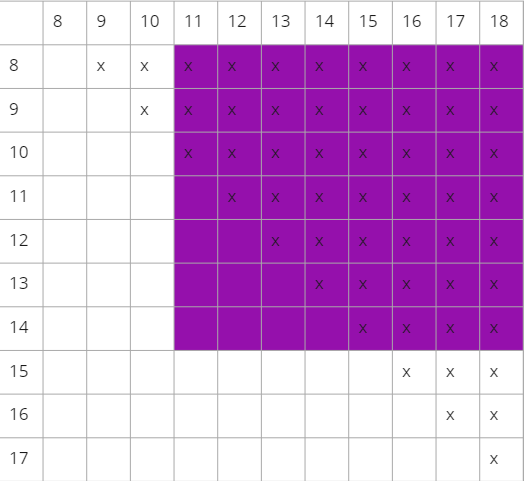
\includegraphics[scale=0.75]{images/matrix_selected.png}
    \caption{Matrix : interferierende Reservierungen markiert}
    \label{fig:matrix_selected}
\end{figure} \par
\newpage
In Zeile \ref{tfm:4} der \texttt{try\_fit}-Methode werden nun die zurückgegebenen Reservierungen nach der X Koordinate sortiert und in die Methode \texttt{find\_first\_valid\_position} übergeben. Diese erfüllt den zweiten Teil des Algorithmus. Mit einer \texttt{foreach}-Scheife wird jede Reservierung durchgelaufen. Es wird die letzte X Position festgehalten und die Distanz der X Position und dem Anfang der Reservierung gemessen. Wenn die Distanz größer oder gleich der Länge der neuen Reservierung, also der Reservierung, welche in das Feld einsortiert werden soll, wird wird die Position zurückgegeben. Andernfalls wir die X Position gleich der X Position des Endes der iterierten Reservierung gesetzt. Wenn keine Distanz gefunden werden kann, wird -1 zurückgegeben, damit die Reservierung aus der Wertung genommen wird.
\begin{lstlisting}[language=python,caption={find\_first\_valid\_position-Methode},captionpos=b,label={lst:ffvp},escapechar=|,numbers=left]
def get_reservation_from_tensor(self, r):
    arr = []

    x_range = self.duration - (r.begin - self.time_range[0])
    x_start = r.begin - self.time_range[0] + 1
    # this must always start at 8 because of this example [8-15] and [9-10] 1 interferes with 2
    y_range = r.ending - self.time_range[0]

    for i in range(x_range):
        for j in range(y_range):
            for reservation in self.tensor[i + x_start][j]:
                arr.append(reservation)

    return arr
\end{lstlisting}
